\section{Database}
The successful operation of the system, proposed in figure \ref{fig:SystemArchitecture}, is entirely dependent on the database, which stores and provides most, if not all, of the content for the application. For a system so dependent on its data, it is crucial that care and appropriate measures are taken when designing the database. In order for the application to be efficient, both in terms of speed and storage, it is essential that the database is designed in a way that minimises storage space by finding an optimal balance of normalisation and redundancy. To ensure data consistency, various degrees of normalisation were used when designing and developing the database. Taking posts as an example, one could store the username and other details of the author along with every post to improve page loading speeds but this would lead to unnecessary redundancy and a significant increase in storage space. As a result of this, the data was split across multiple tables, based on attributes, which relied on each other through the use of functional dependencies and relationship constraints to ensure consistency and provide a complete dataset. An overview of the database is provided in section \ref{SubSection:Database_Schema} along with a breakdown of the tables based on components of the system in section \ref{SubSection:Database_Tables}. An explanation of the normalisation techniques and dependencies is also provided in sections \ref{SubSection:Database_Normalisation} and \ref{SubSection:Database_Constraints} respectively.

\subsection{Schema}
\label{SubSection:Database_Schema}
In line with the agile methodology and component driven design approach adopted for the development of the project, the database was also designed with modularity in mind. This allows the database to be expanded as new system components were developed. Each component stores its data in independent tables which rely on previously implemented tables through relational dependencies. The diagram in figure \ref{fig:Database_ERD} shows the set of tables in the database, and the relationship between these tables, at the time of documentation. There are currently 21 tables in the database but these do not represent 21 components as some components encapsulate multiple tables. The design of each table and the choices made are discussed in section \ref{SubSection:Database_Tables}, categorised by components.

There are some consistent attributes across all the tables shown in the diagram. The id column is used as a primary key to provide each tuple with a unique identifier. This primary key is used to manipulate the row based on user input, such as editing and deleting. The last three columns store the date on which the tuple was created, updated, and deleted respectively. The created at column is never updated after the record has been created. The updated at field is changed to the current timestamp whenever the record is changed, e.g. if a user changes their password or the system updates a users reputation. The deleted at column will be null by default, until the user deletes the tuple. This is used for the soft delete feature to prevent it from being selected without actually removing it \cite{PCMEncyclopedia:SoftDelete}.

\begin{figure}[H]
  \centering
  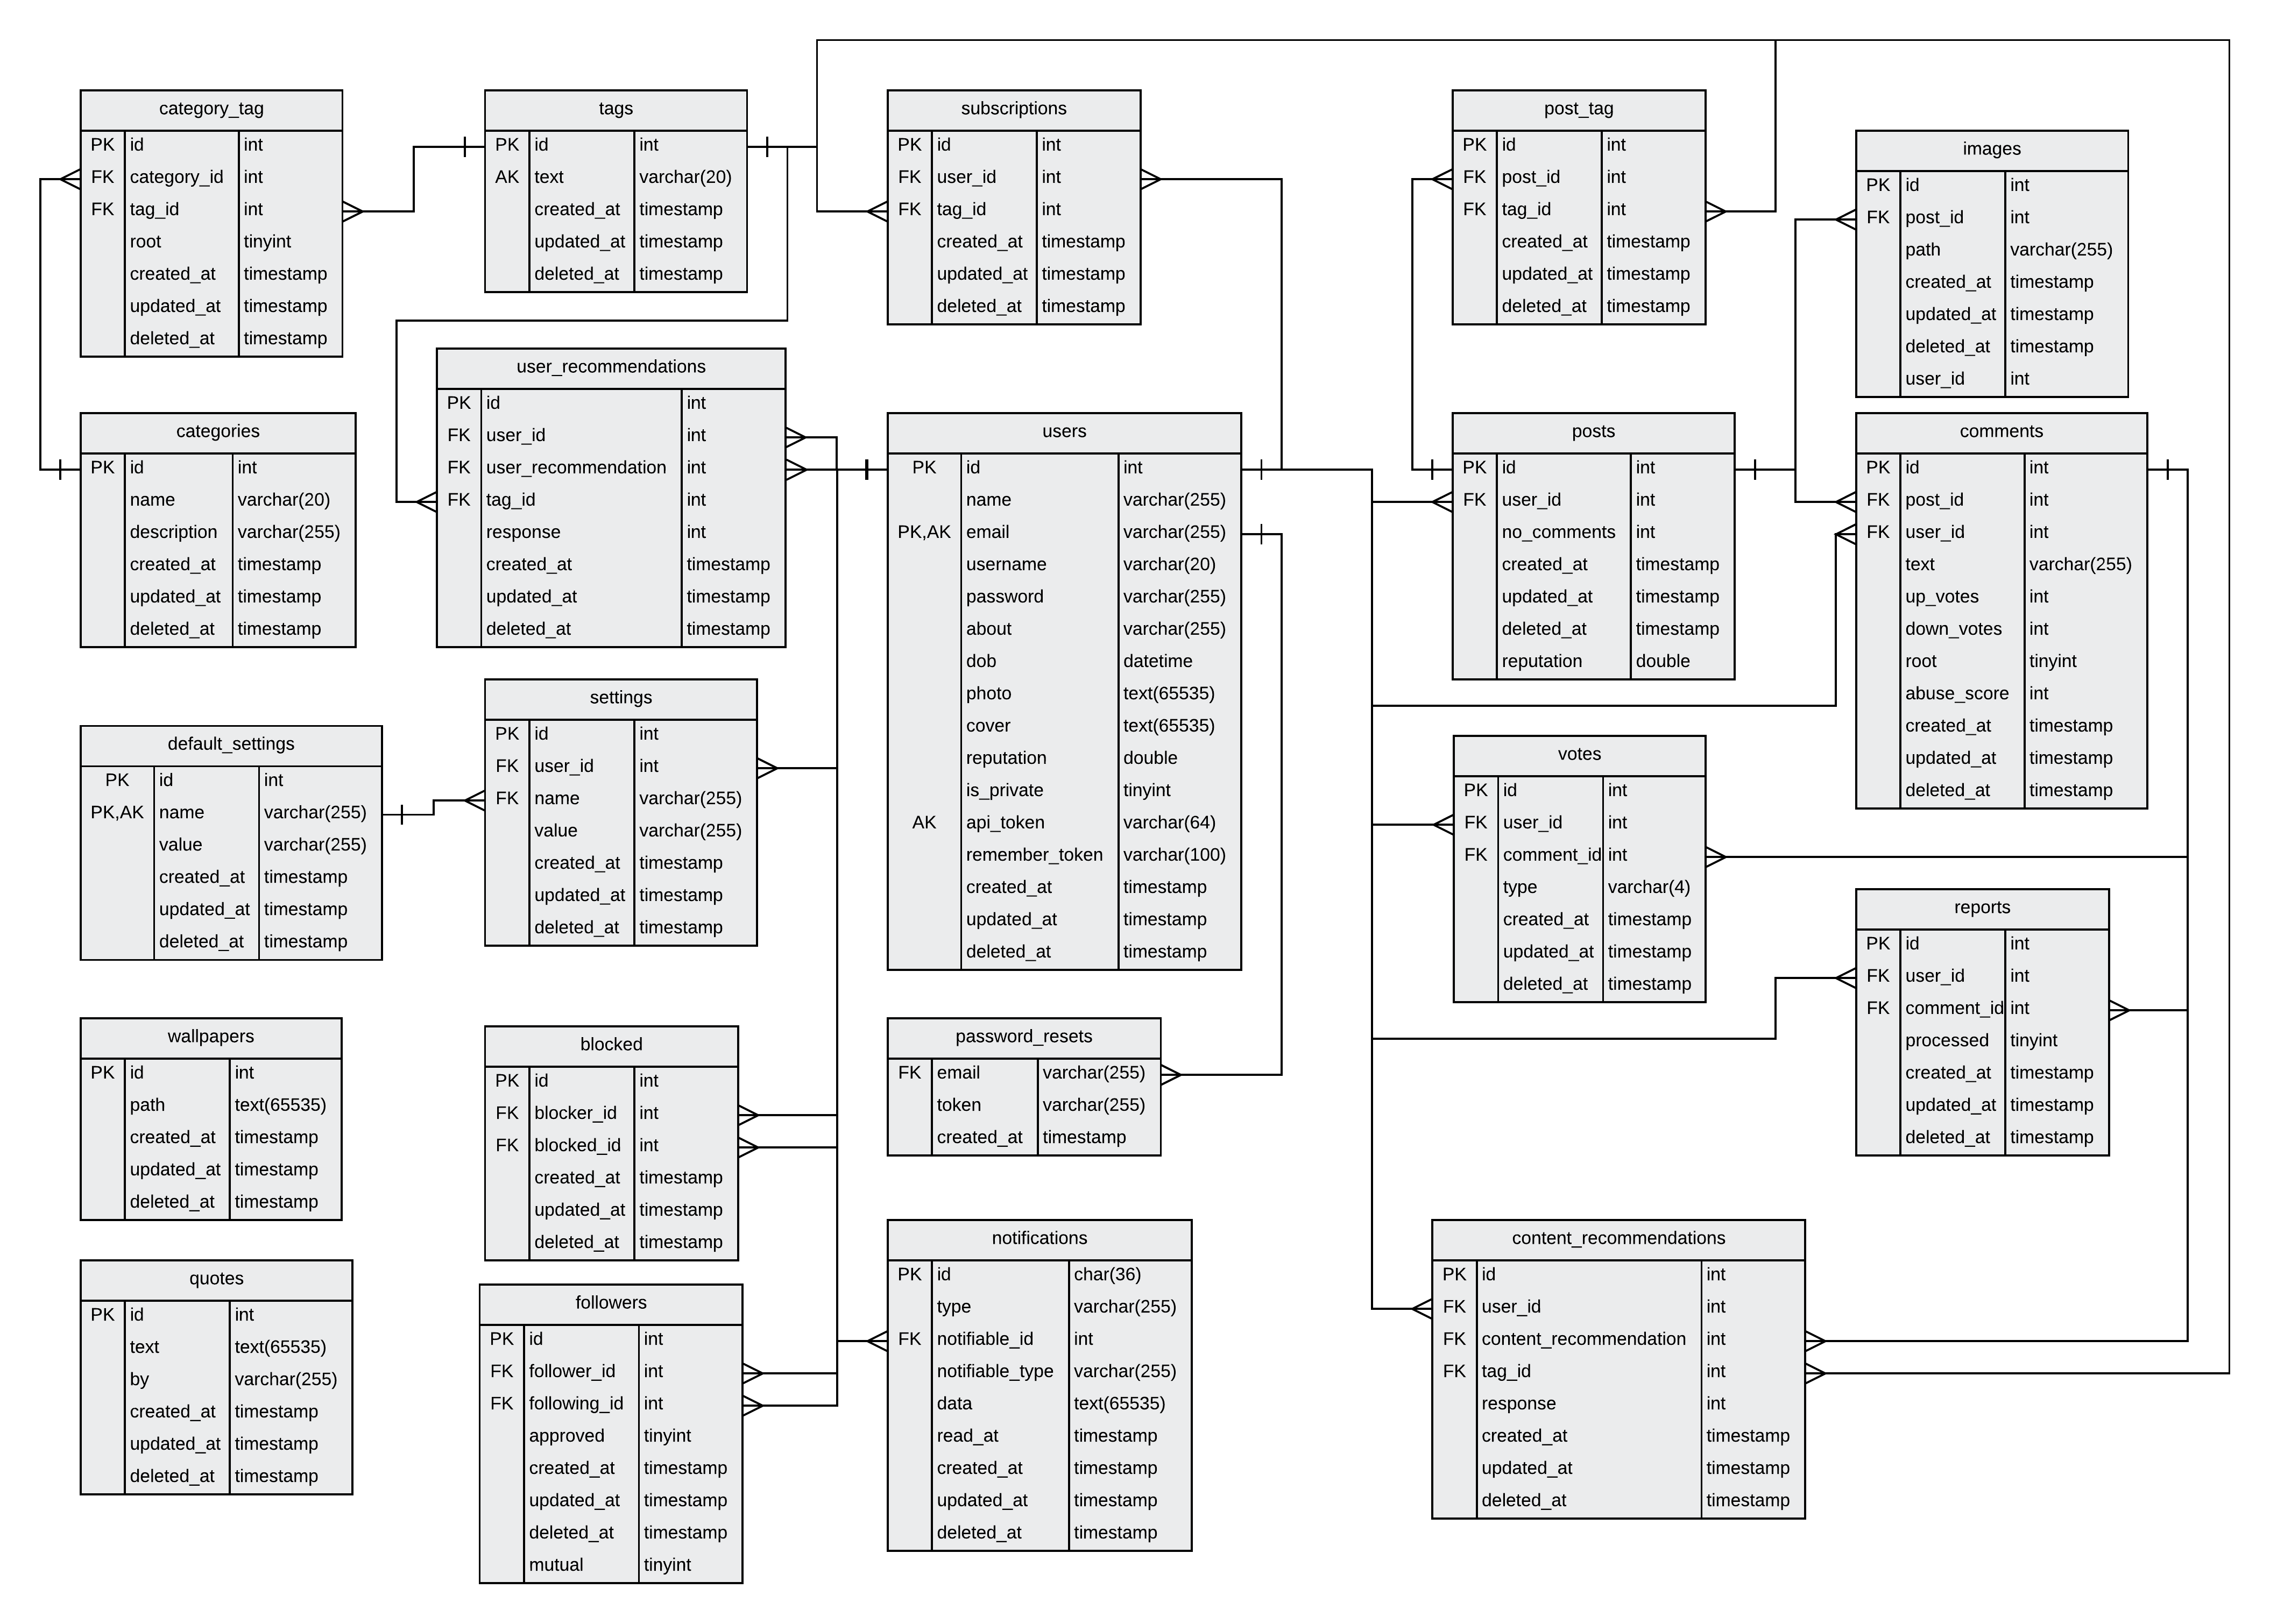
\includegraphics[width=1.0\textwidth]{Images/Design/Database/ERD}
  \caption{Database Schema Represented as an Entity Relationship Diagram (ERD).} \label{fig:Database_ERD}
\end{figure}

\subsection{Tables}
\label{SubSection:Database_Tables}
As mentioned previously, the database consists of many tables comprising many components of the systems. The design of each of the tables, categorised by components, is discussed in this section.

\subsubsection{User and Authentication}
The user is one of the core components of the system. A significant amount of the functionality provided by the system, including but not limited to the authentication system, is reliant upon the user table. This can be seen be the dependencies on the user table in figure \ref{fig:Database_ERD}. Despite the fact that the users details are stored in just one detail, the entire component is comprised of two tables due to the authentication mechanism. The main table which hold the user data is called `users'. Along with its primary key field, id, it also has a primary key on the email field and an alternate key on the email and api token field. This will allow for quick fetching of the user using the api token field when accessing the API. The second table comprising the authentication mechanism is the password resets table which stores recovery tokens when the user makes a forgotten password request. Unlike the other tables, this table does not have an id field but instead it has a foreign key, email, relating a recovery token to the user who requested it. This constraint is also the reason for the index on the email field in the users table.

\begin{figure}[H]
  \centering
  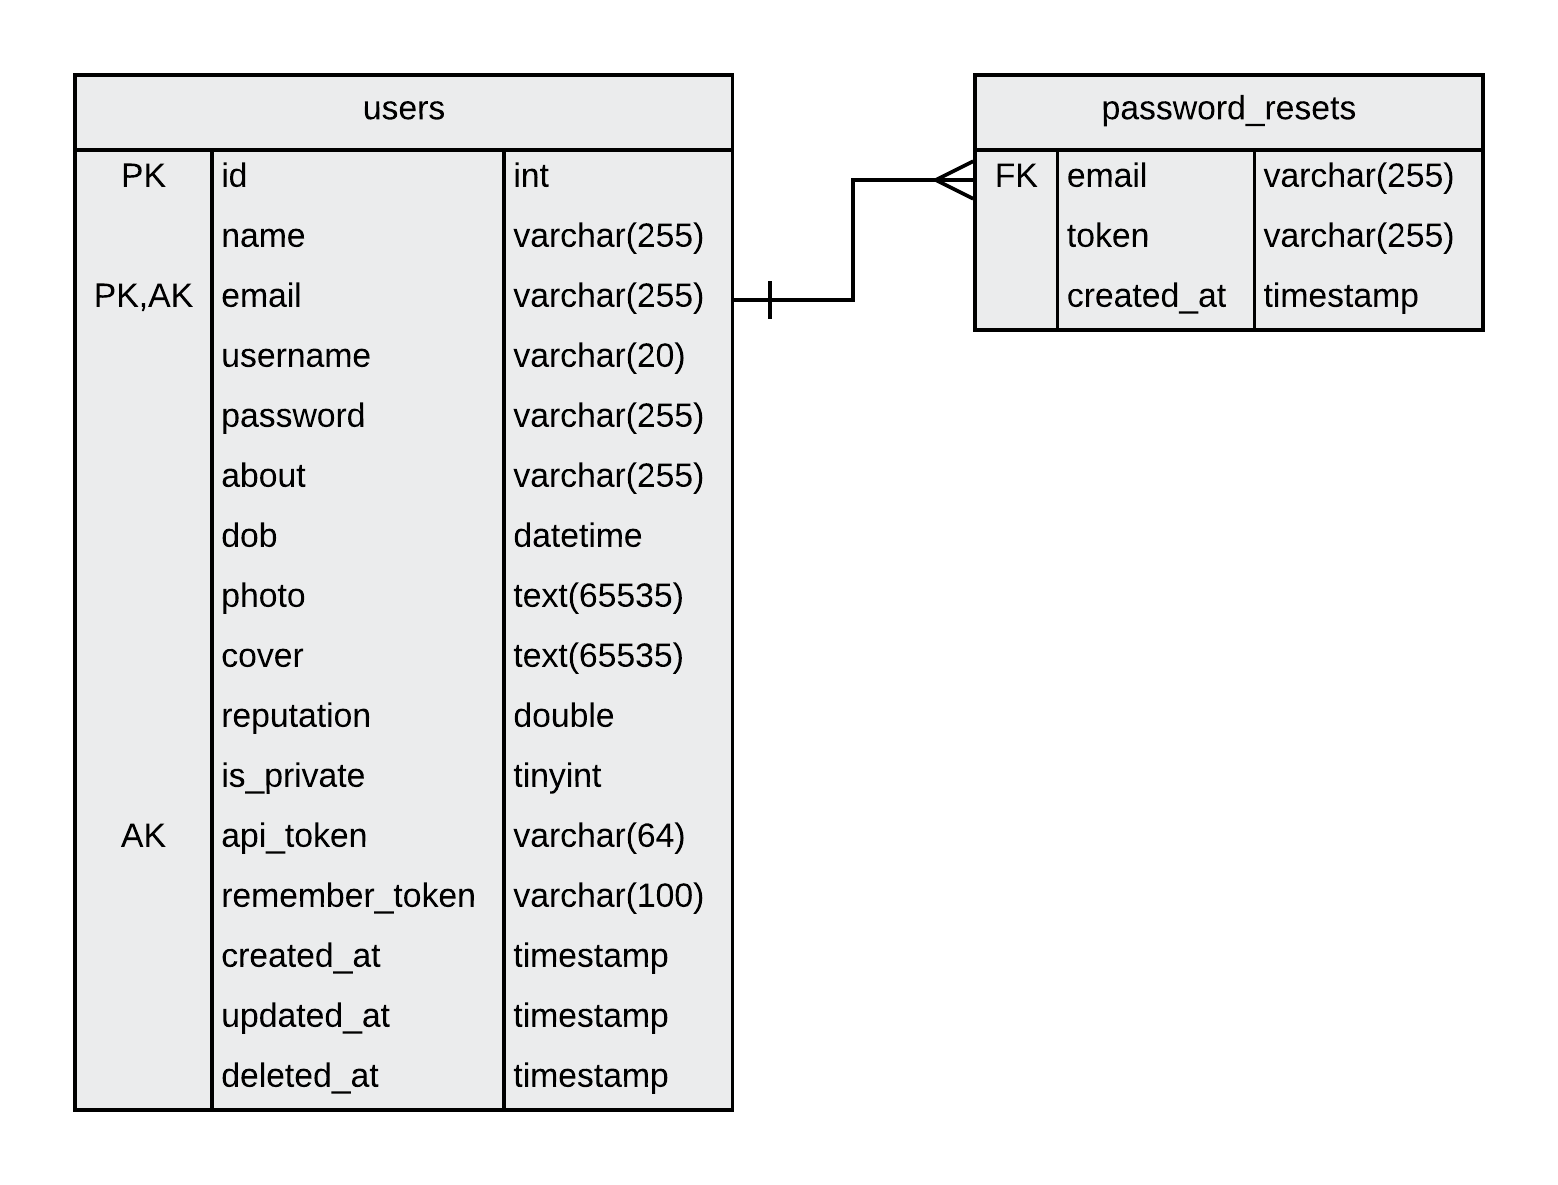
\includegraphics[width=1.0\textwidth]{Images/Design/Database/Users}
  \caption{Entity Relationship Diagram - Users and Authentication} \label{fig:ERD_Users}
\end{figure}

\subsubsection{Settings}
Each user will have various settings which they will tune to customise their social network and the way they see information. One way of storing these settings would be to add a new column in the user table for every setting. However this is not the best approach as it would mean continuously updating the users table and the code for inserting and fetching data from this table.

Another approach for storing the settings for each user would be to create a settings table which acts like a dictionary with a key and value column, where the key is the name of the setting. Each row would then be mapped to a user indicating which settings belong to a specific user. The problem encountered with this approach is that when a new user registers, a record for every setting would have to be inserted in the settings table. Once again, this would complicate the process of adding new settings as they would have to be added via code. Additionally, a new record would have to be added for every existing user for this new setting.

In the final design, the second approach along with an additional default settings table was created. This allowed the process of adding new settings to be simplified and reduced a significant amount of redundant data. Most users on the system will use the default browsing experience or only tweak a handful of settings making it unnecessary to replicate every setting for them. Using the default settings table meant that new settings could easily be created by simply adding a new row. Additionally, it also meant that for every user the default settings could be loaded and only settings they changed would be stored in the settings table and loaded to override the default settings.

An alternative primary key index was added to the name field in the default settings table. This allowed for quick fetching of a default setting by name. A foreign key index on the name field in the settings table which referenced the name field in default settings ensured that only settings defined in the default settings table could exist in the users custom settings table.

\begin{figure}[H]
  \centering
  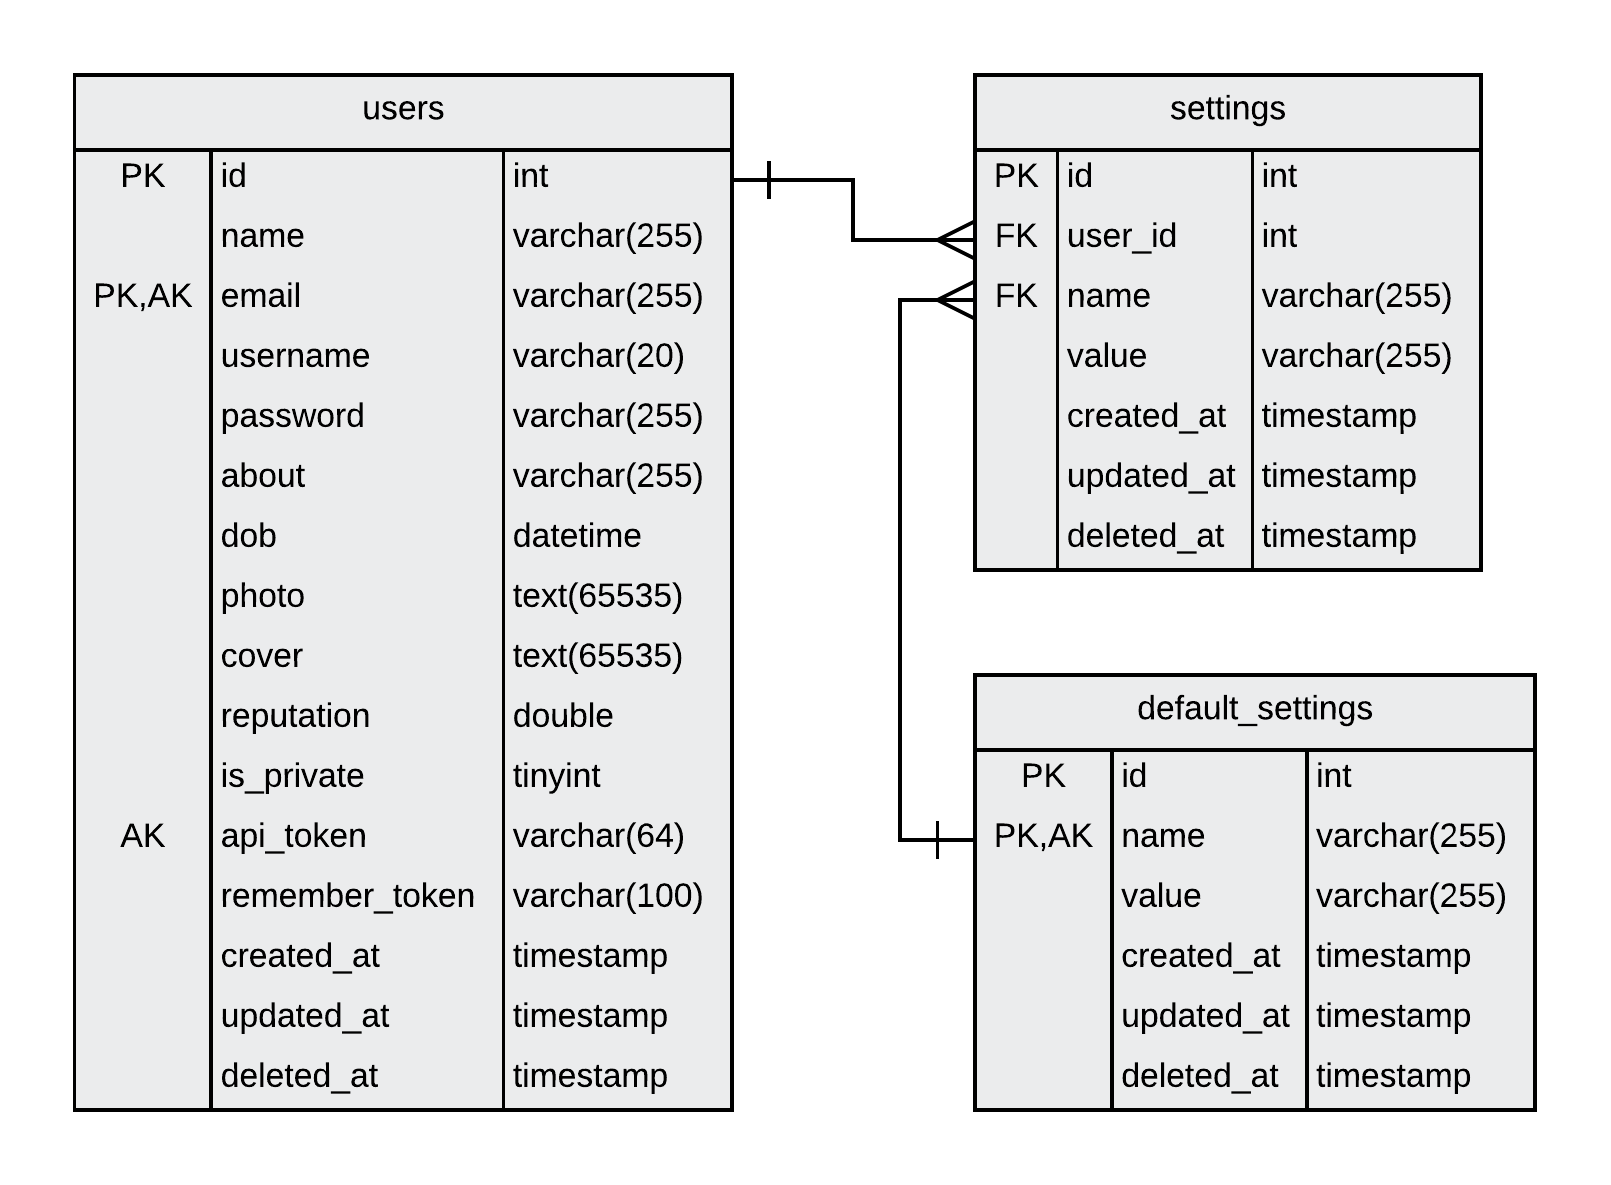
\includegraphics[width=1.0\textwidth]{Images/Design/Database/Settings}
  \caption{Entity Relationship Diagram - User Settings} \label{fig:ERD_Settings}
\end{figure}

\subsubsection{Following and Blocking}

For the social network to work and provide personalised content from familiar faces, users need the ability to follow one another. To provide this functionality, it is necessary to store the relationships between the various users. A followers table was created for exactly this purpose. The follower id field stores the user that is following and the following id contains the user that is being followed. Both these fields are foreign keys which reference the users table to indicate the users in a relationship. As a user may have a private and would like to control who follows them, an approved field was added which stores a boolean value. As development progressed, a mutual field was added to indicate a two way relationship.

Often abusive users will spam the content posted by the users they follow. As there is no way to prevent a user from following you if your profile is public, an additional feature was required. This feature allows users to block other uses, preventing the blocked user from being able to see the blockers profile and preventing both users from seeing each others content on their feed. The blocked table, similar to the followers table, contains the id of the blocker and the person being blocked with both referencing the user table.

\begin{figure}[H]
  \centering
  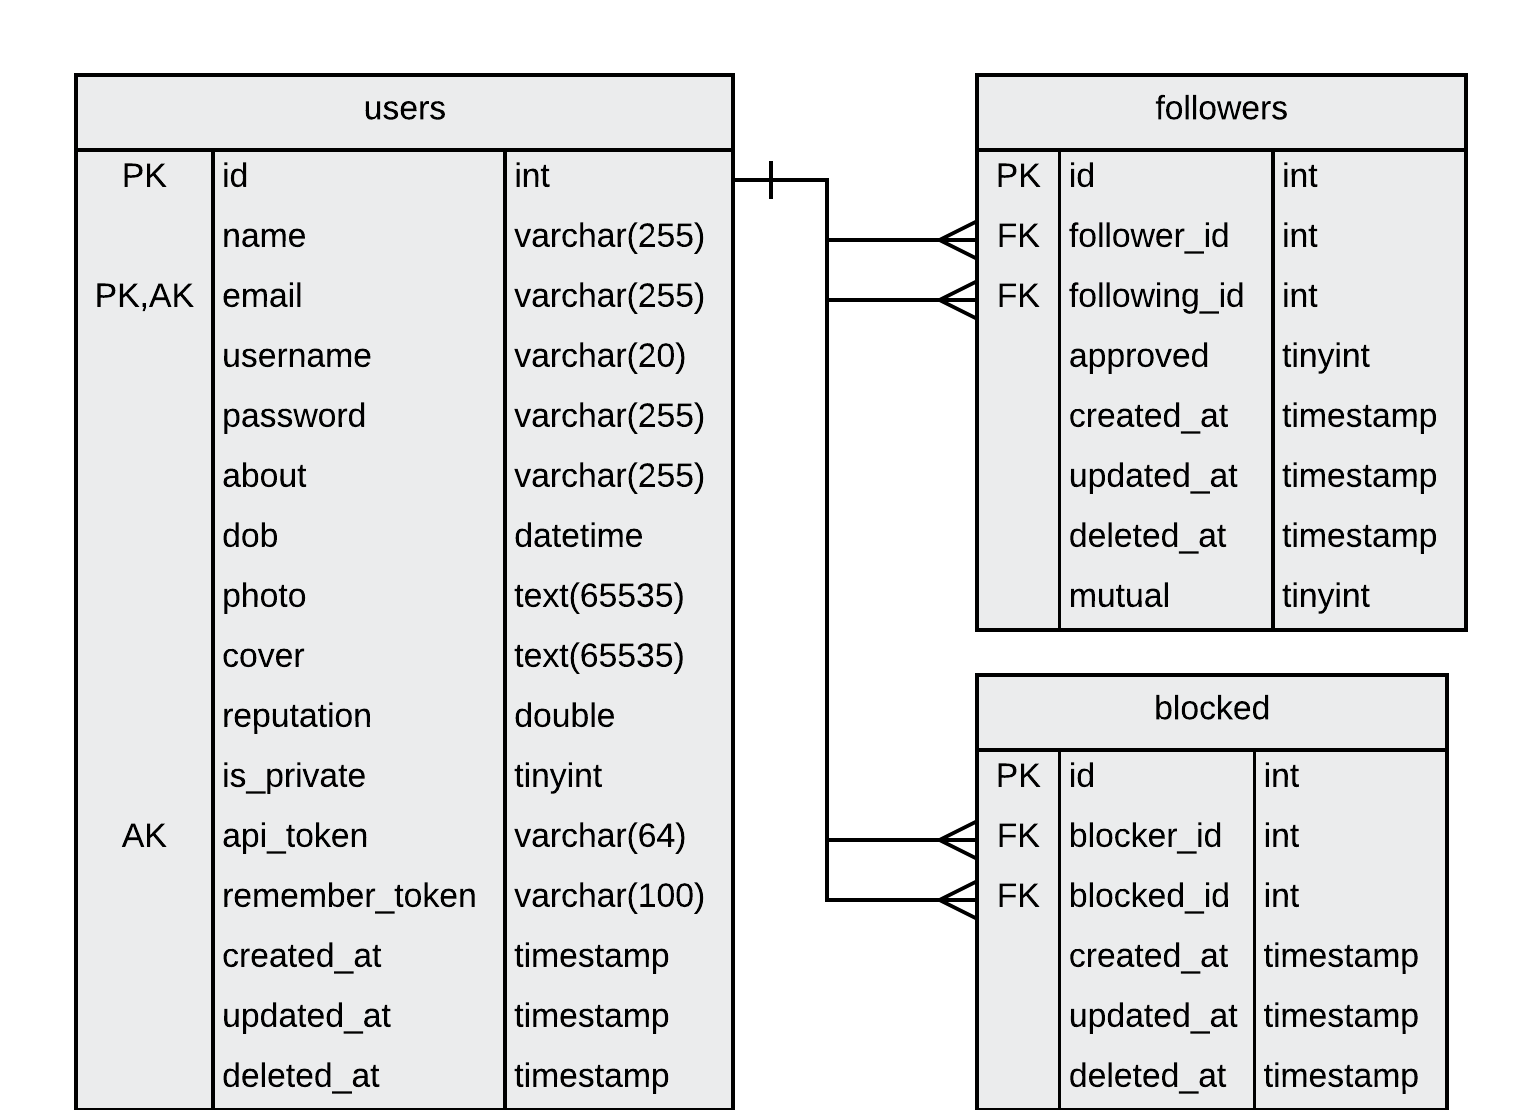
\includegraphics[width=1.0\textwidth]{Images/Design/Database/Followers}
  \caption{Entity Relationship Diagram - Users Followers and Blocked} \label{fig:ERD_Followers}
\end{figure}

\subsubsection{Categories and Tags}
Every post should ideally be categorised into a specific category or even a set of categories. Users can tag their posts manually or allow the categorisation algorithm to do it for them. The issue faced here is that categories are ever evolving and users define new tags every day. To make the process of creating categories easier and store all this tag data, three separate tables were designed. 

\paragraph{Tags}
The tags table is completely independent of every other table in the database. It simply stores the text that makes up a tag and indexes this field so that tags can quickly be received using their text value.

\paragraph{Categories}
As with the tags table, this table is completely independent of all others in the database. The difference with this table is that it will contain only a subset of tags which all other tags can be categorised into. Additionally, a description is also added for each tag in this table.

\paragraph{Category Tag}
This table is a kind of pivot table between categories and tags. The only purpose of this table is to link each tag to a category in the categories table. A tag may be linked to multiple categories hence the one to many relation from the tags to this pivot table. A root field is also added to this table which indicates that the tag has same the text value as the category name. For example, the tag `Politics' would be considered a root for the `Politics' category but it would also fall under the `News' category.

\begin{figure}[H]
  \centering
  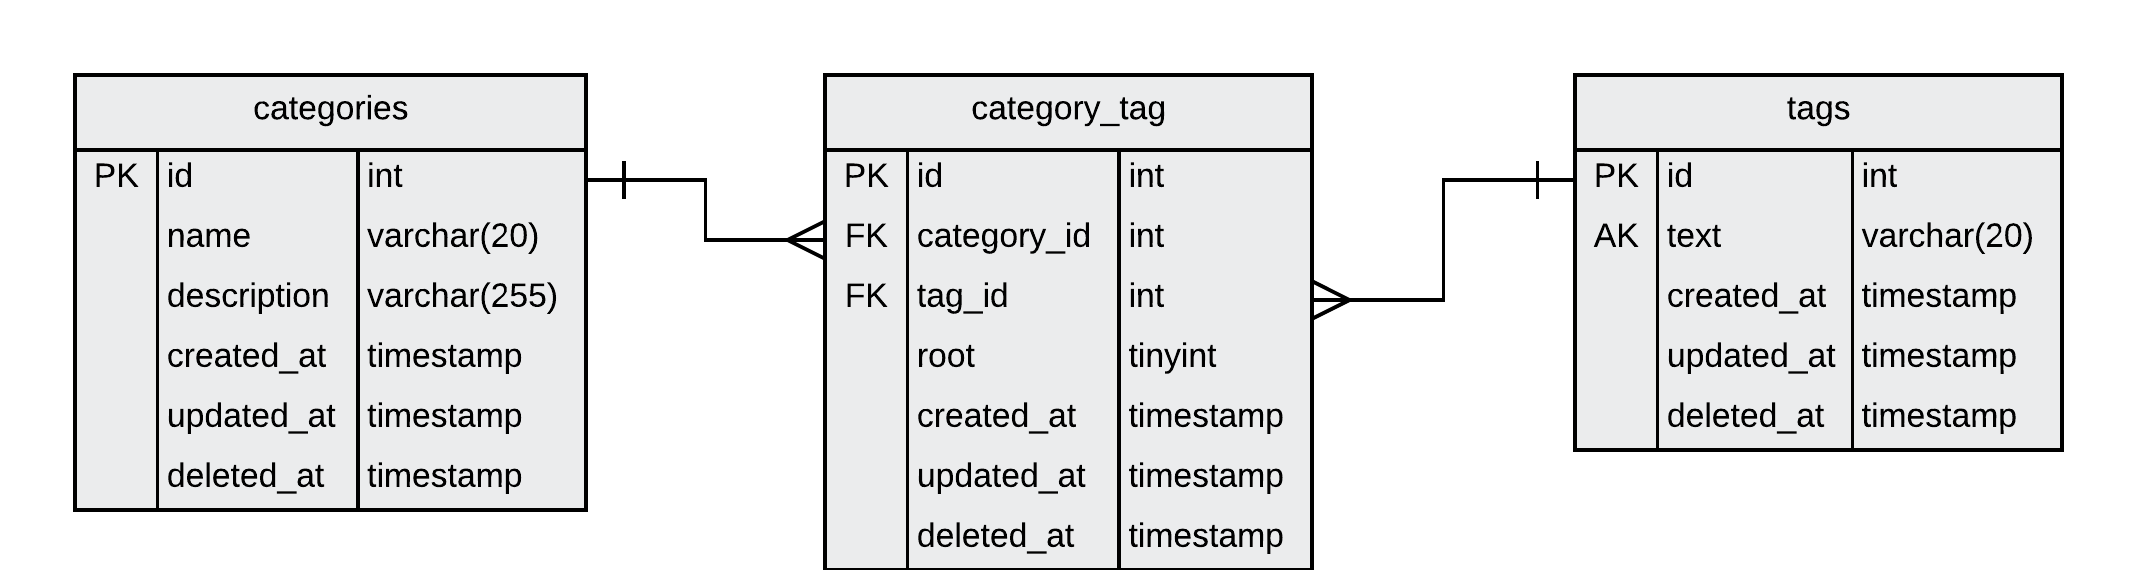
\includegraphics[width=1.0\textwidth]{Images/Design/Database/Categories}
  \caption{Entity Relationship Diagram - Categories and Tags} \label{fig:ERD_Categories}
\end{figure}

\subsubsection{Subscriptions}
The subscriptions table is responsible for storing the relationship between a user and a tag or many tags. For this reason, the subscriptions table simply stores a user id along with a tag id for each record. Each record indicates the user that is subscribed to a specific tag. As a user may subscribe to multiple tags and a tag may be subscribed to by multiple users, a one to many relationship is used from the users and tags table to the user id and tag id fields respectively.

\begin{figure}[H]
  \centering
  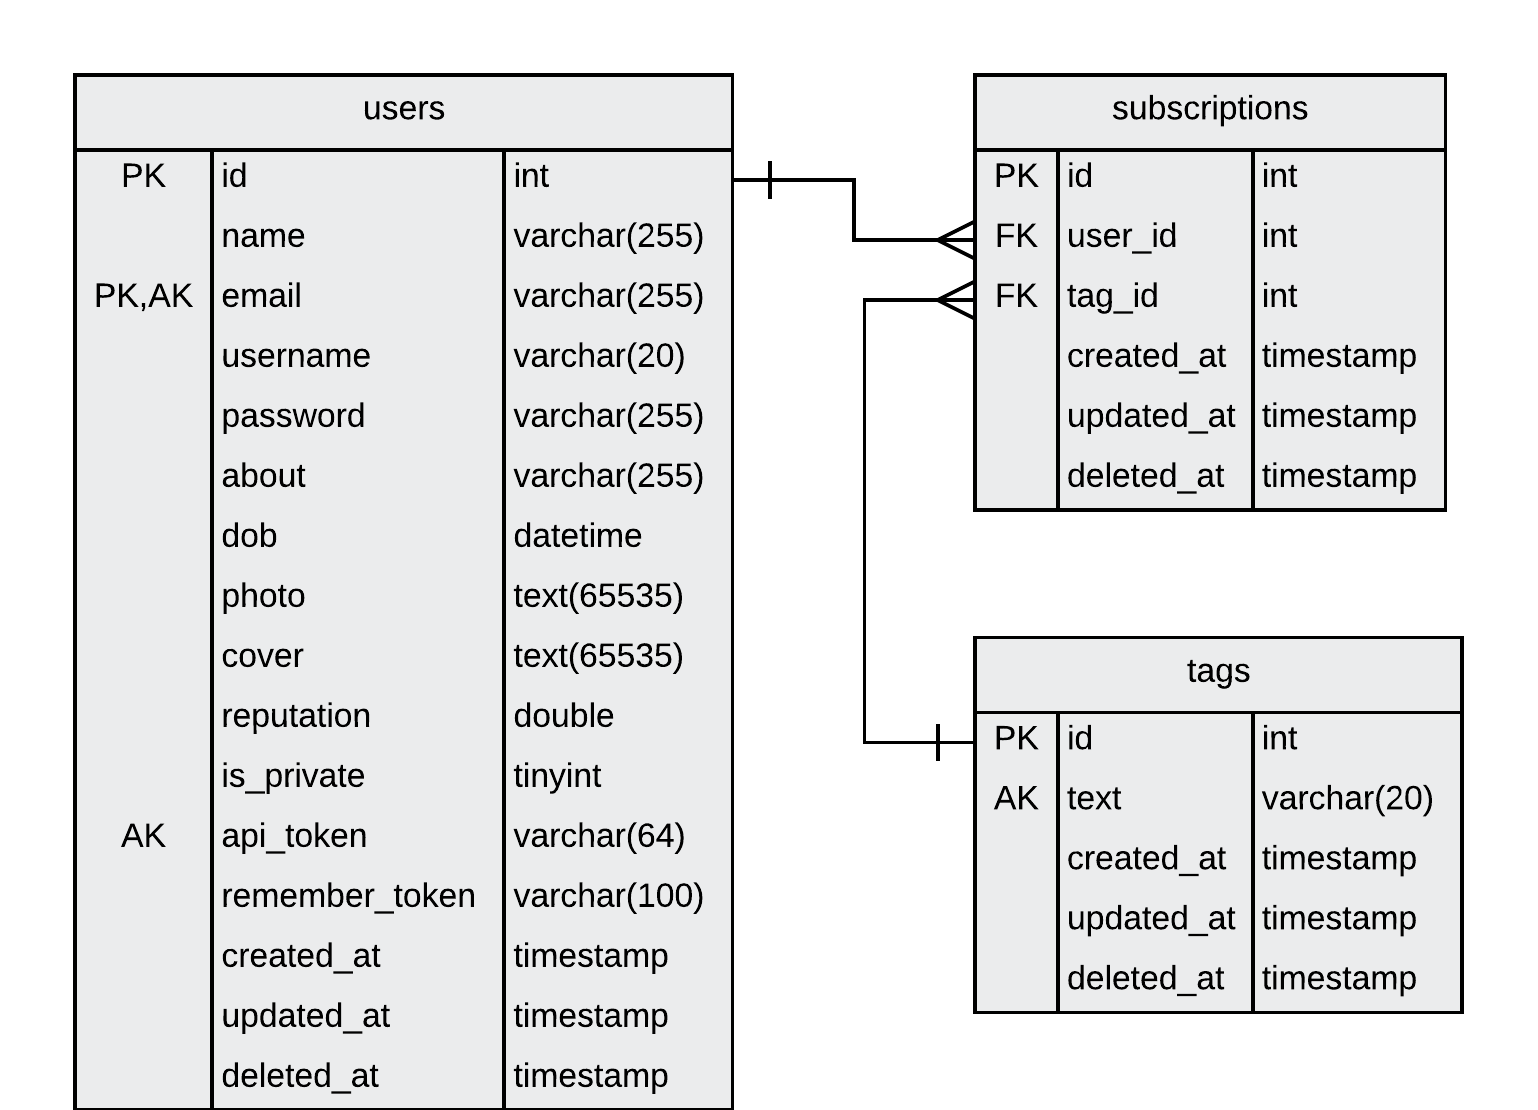
\includegraphics[width=1.0\textwidth]{Images/Design/Database/Subscriptions}
  \caption{Entity Relationship Diagram - Users Subscribed Tags} \label{fig:ERD_Subscriptions}
\end{figure}

\subsubsection{Posts and Comments}
Being able to efficiently store posts, comments, and images is one of the core features of any social network. In order to store posts in fidelis, a posts table was created which contained the user id, the post text, the number of comments, the number of up and down votes and the abuse score. These fields encapsulated all the required data to display a post to other users.

In order to provide the comment functionality, an additional comments table was created. This table, much like the posts table, stored the user id, the comment text, the number of up and down votes and the abuse score along with the post id. At this point it became clear that there were too many similarities between the posts and comments table which added unnecessary complexity. To resolve this and make the design more efficient, duplicate attributes across the tables were removed from the post table. Now, instead of storing posts in the posts table, an empty post would be created along with a comment which stored the post text. As a result, a root field was introduced to indicate the root comment for a post.

Posts also have additional features which comments do not have. For example, posts can have images and can be categorised using tags. This is the primary reason that the post table was not removed entirely. An images table was created which mapped the path of the uploaded image(s) to the post which the images belong to. Similarly, a post tag table maps all the tags which have been applied in the post text to the post.

Figure \ref{fig:ERD_Posts} shows the proposed table structure and how the posts and comments table were broken down. An additional reputation field was added to the posts table to maintain the reputation score computed based on all the interactions with the post and its comments.

\begin{figure}[H]
  \centering
  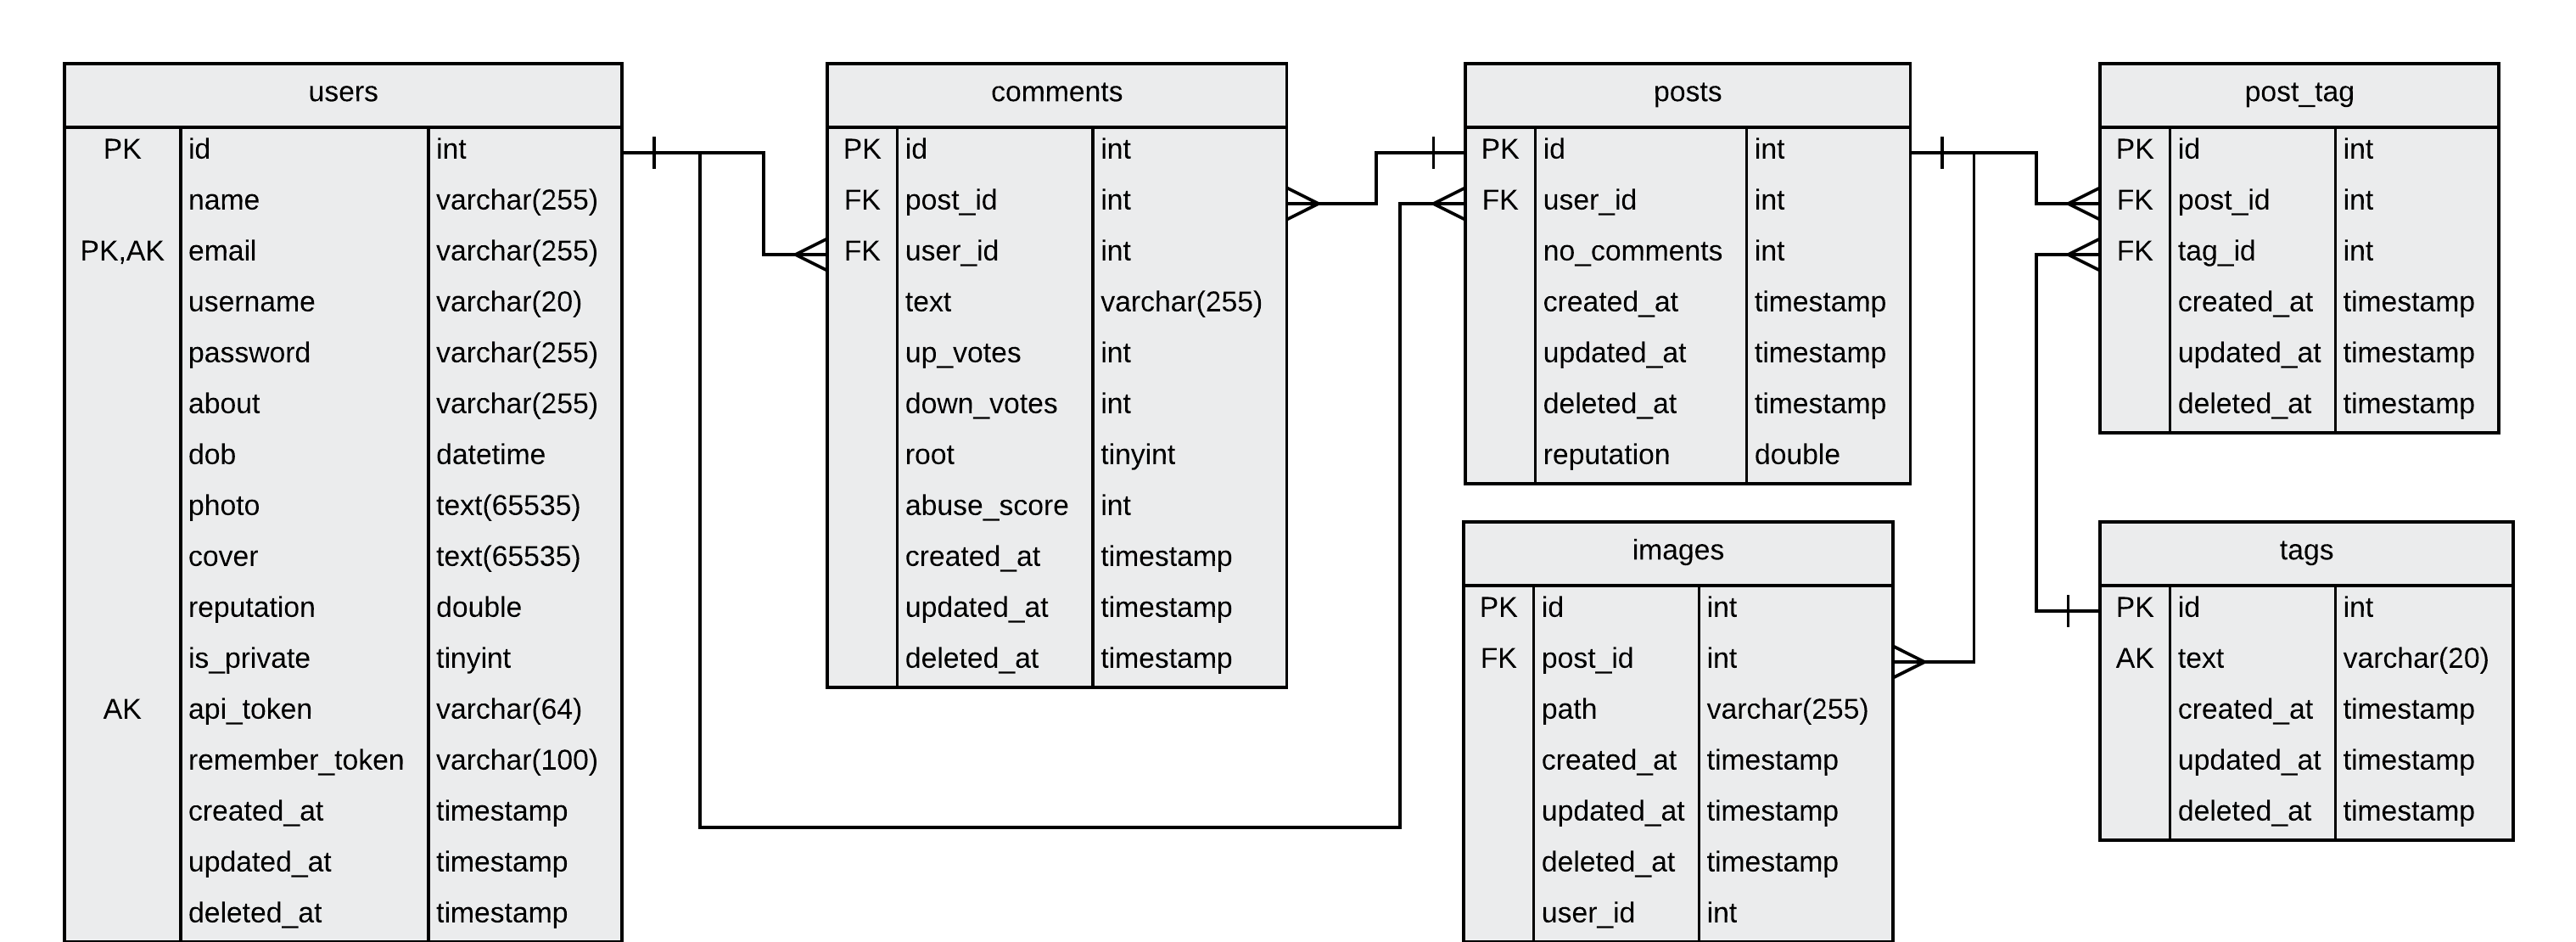
\includegraphics[width=1.0\textwidth]{Images/Design/Database/Posts}
  \caption{Entity Relationship Diagram - Users Posts and Comments} \label{fig:ERD_Posts}
\end{figure}

\subsubsection{Voting}
The functionality for voting will be maintained by just one table. The votes table is very minimal, containing just the user id, comment id and the type of vote. The user id and comment id have a one to many relation to the users and comments table respectively as a user many vote on multiple posts and multiple users may vote on one post. The type field can either hold a positive value or a negative value, indicating likes and dislikes respectively.

\begin{figure}[H]
  \centering
  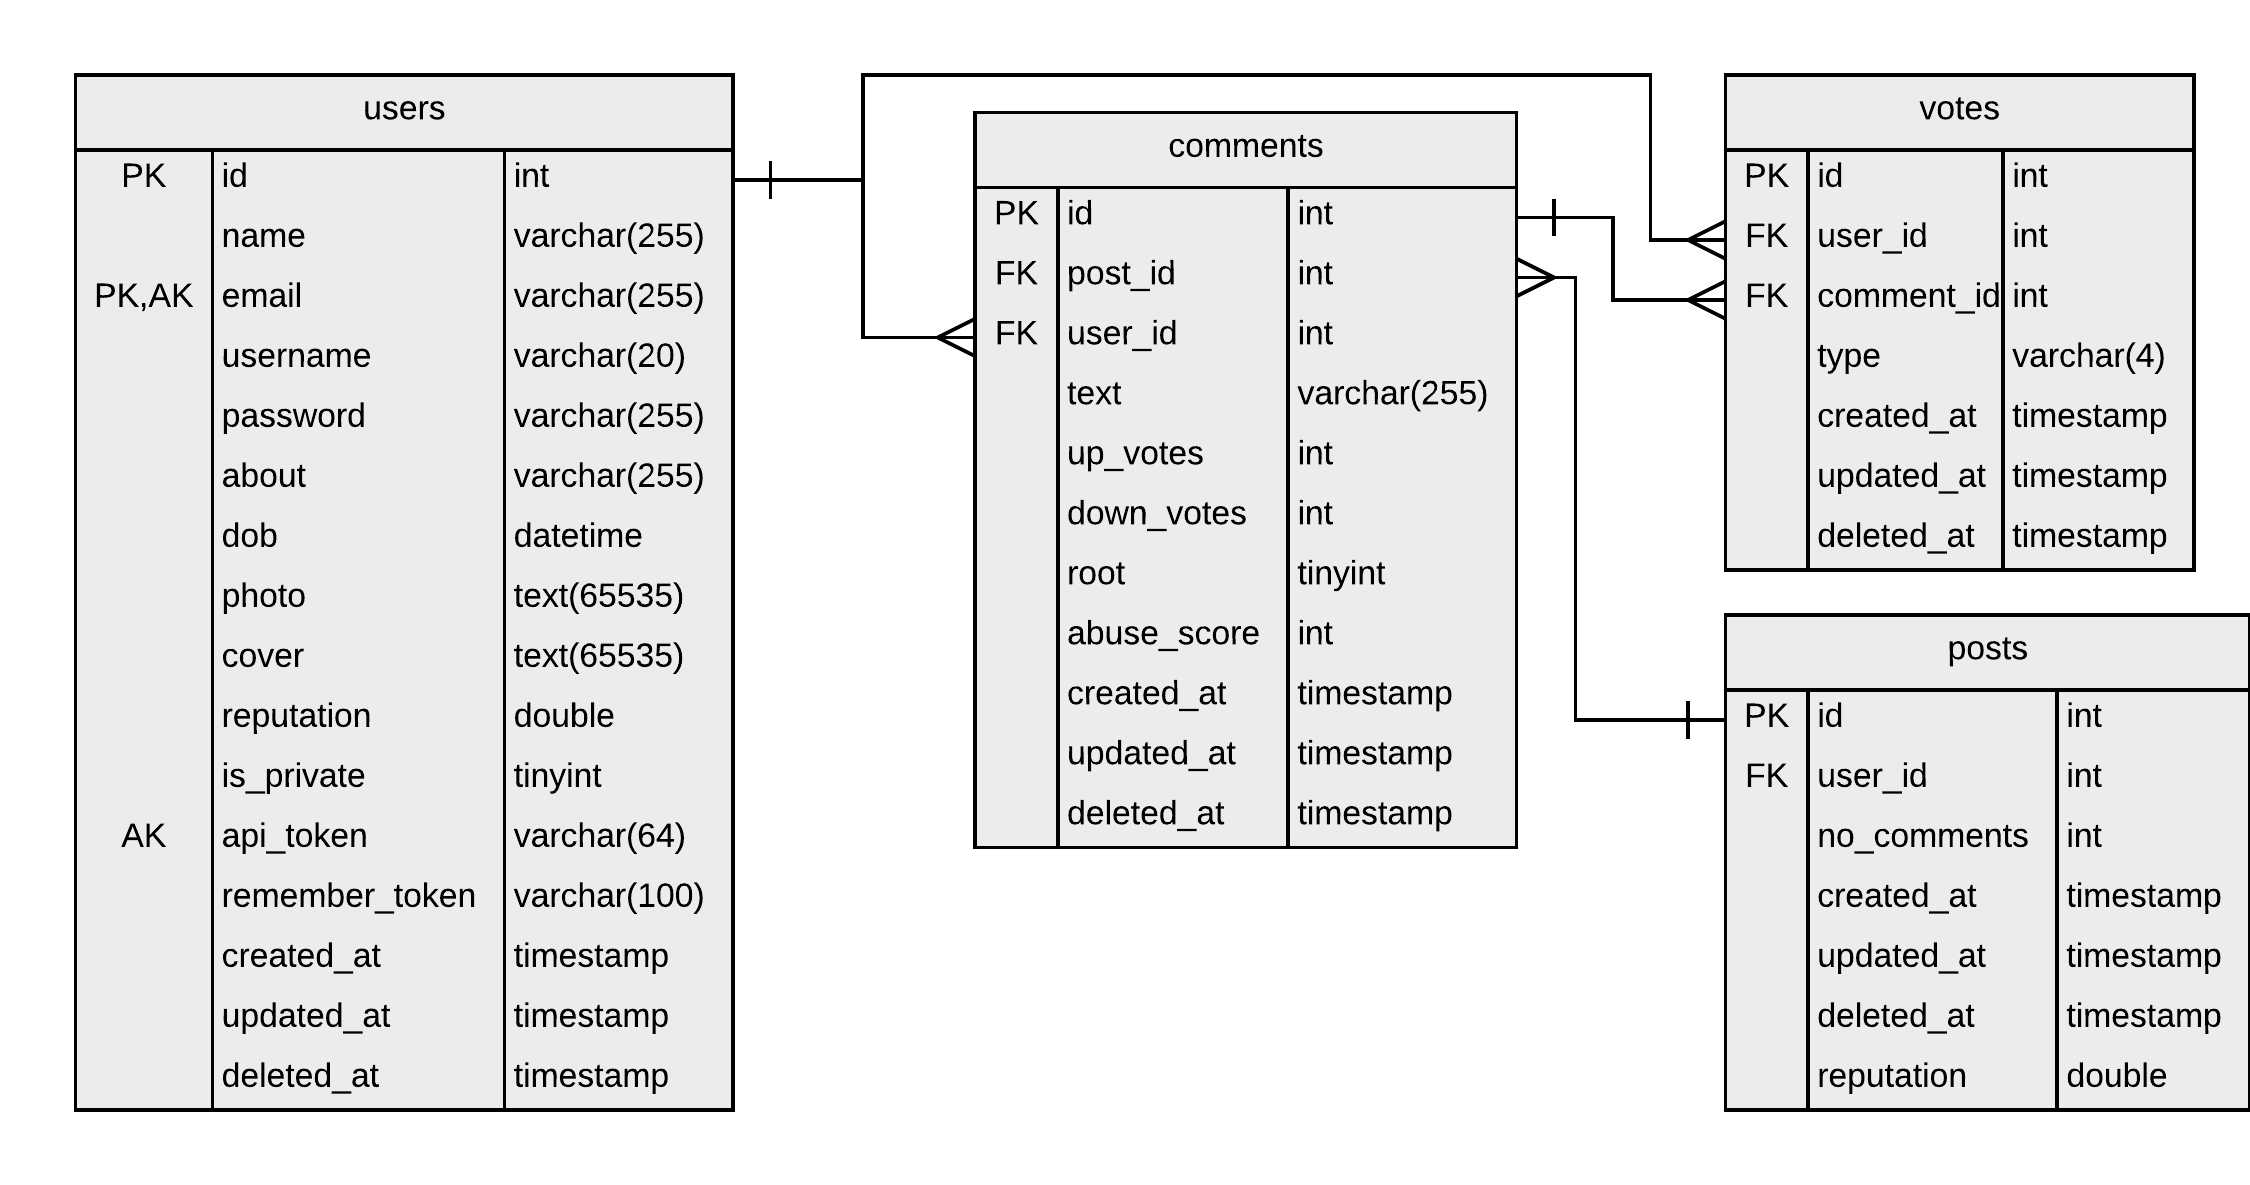
\includegraphics[width=1.0\textwidth]{Images/Design/Database/Votes}
  \caption{Entity Relationship Diagram - Voting on Posts and Comments} \label{fig:ERD_Voting}
\end{figure}

\subsubsection{Reporting}
Reporting a post is the next step to voting. Ideally, if a user finds a post irrelevant or offensive, they will dislike it which will recommend less of similar content. However, if a user finds something extremely abusive then, they can report the content to be removed or hidden. This functionality is also provided by just one table. The table, like votes, contains a user id and comment id which have a one to many relation to the users and comments table respectively as a user many report multiple posts and multiple users may report one post. Additionally, a processed boolean field is used to indicate the status of a report. 

\begin{figure}[H]
  \centering
  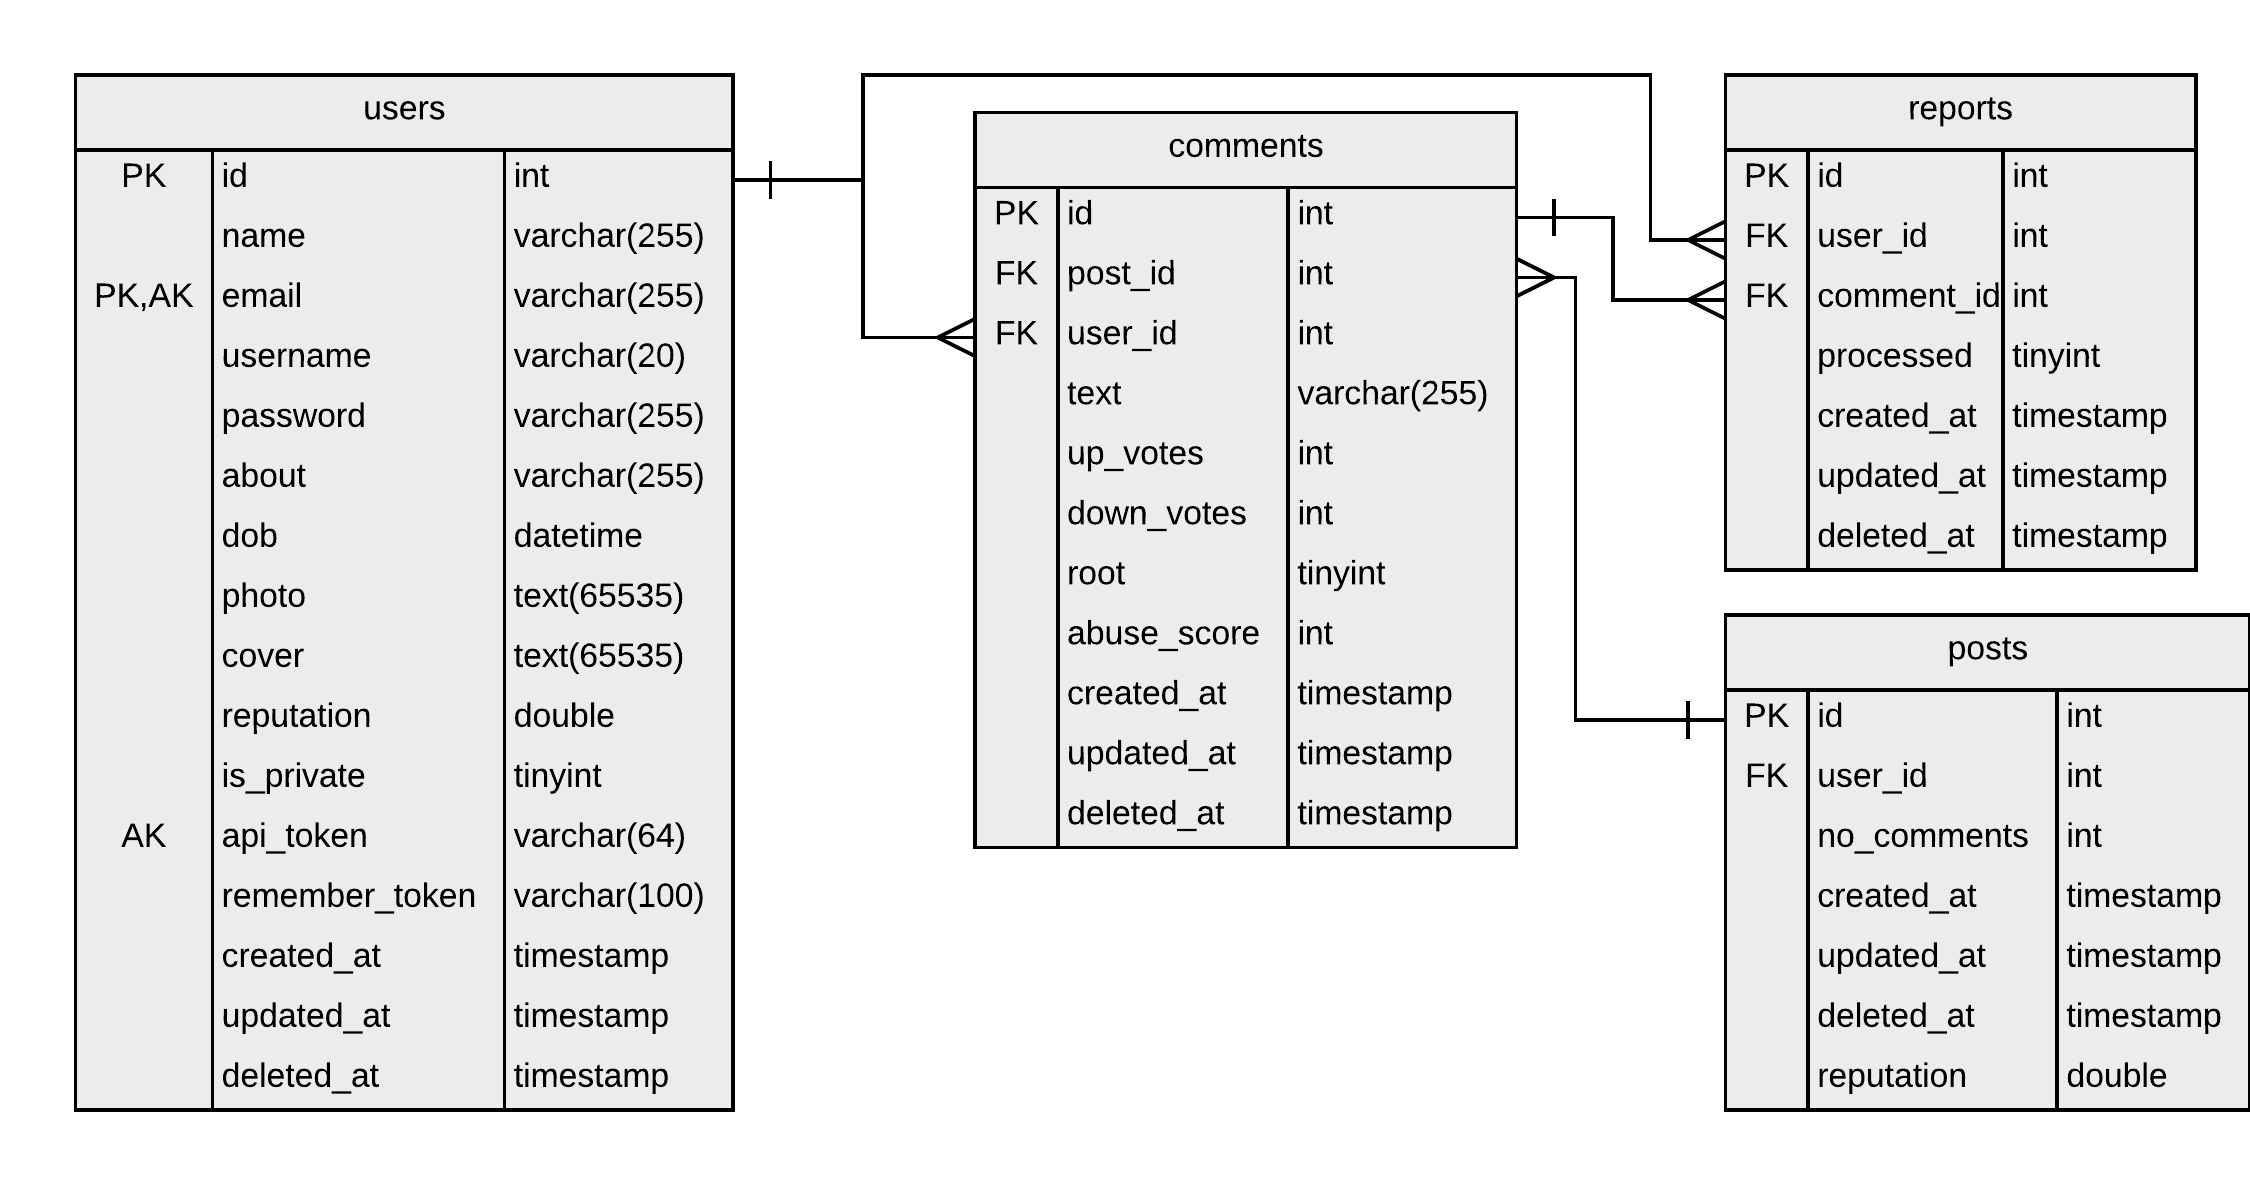
\includegraphics[width=1.0\textwidth]{Images/Design/Database/Reports}
  \caption{Entity Relationship Diagram - Reporting Posts and Comments} \label{fig:ERD_Reporting}
\end{figure}

\subsubsection{Notifications}
Designing a table for the notification system was particularly tricky. A notification will always be intended for a specific person but it may be regarding various types of interactions. For example, a notification could be about a new follower in which case it is regarding a user or it could be about a vote in which case it is regarding a comment. This made it difficult to store the content which the notification is about with an index to the corresponding table. As a result, the notifications table contained a type field indicating the type of notification, e.g. 'comment' or 'vote'. The notifiable id field has a one to many relationship from the users table as a user may receive many receive many notifications. The notifiable type field stores the model which the notification is for, which for the moment will always be a user but in the future may be a guest or other values. The data field contains the notification data which is comprised of the text and the id of the content it concerns. The downside of this approach is that an index cannot be added on the id of the content to ensure integrity and consistency but the generic advantages outweigh the cons.

\begin{figure}[H]
  \centering
  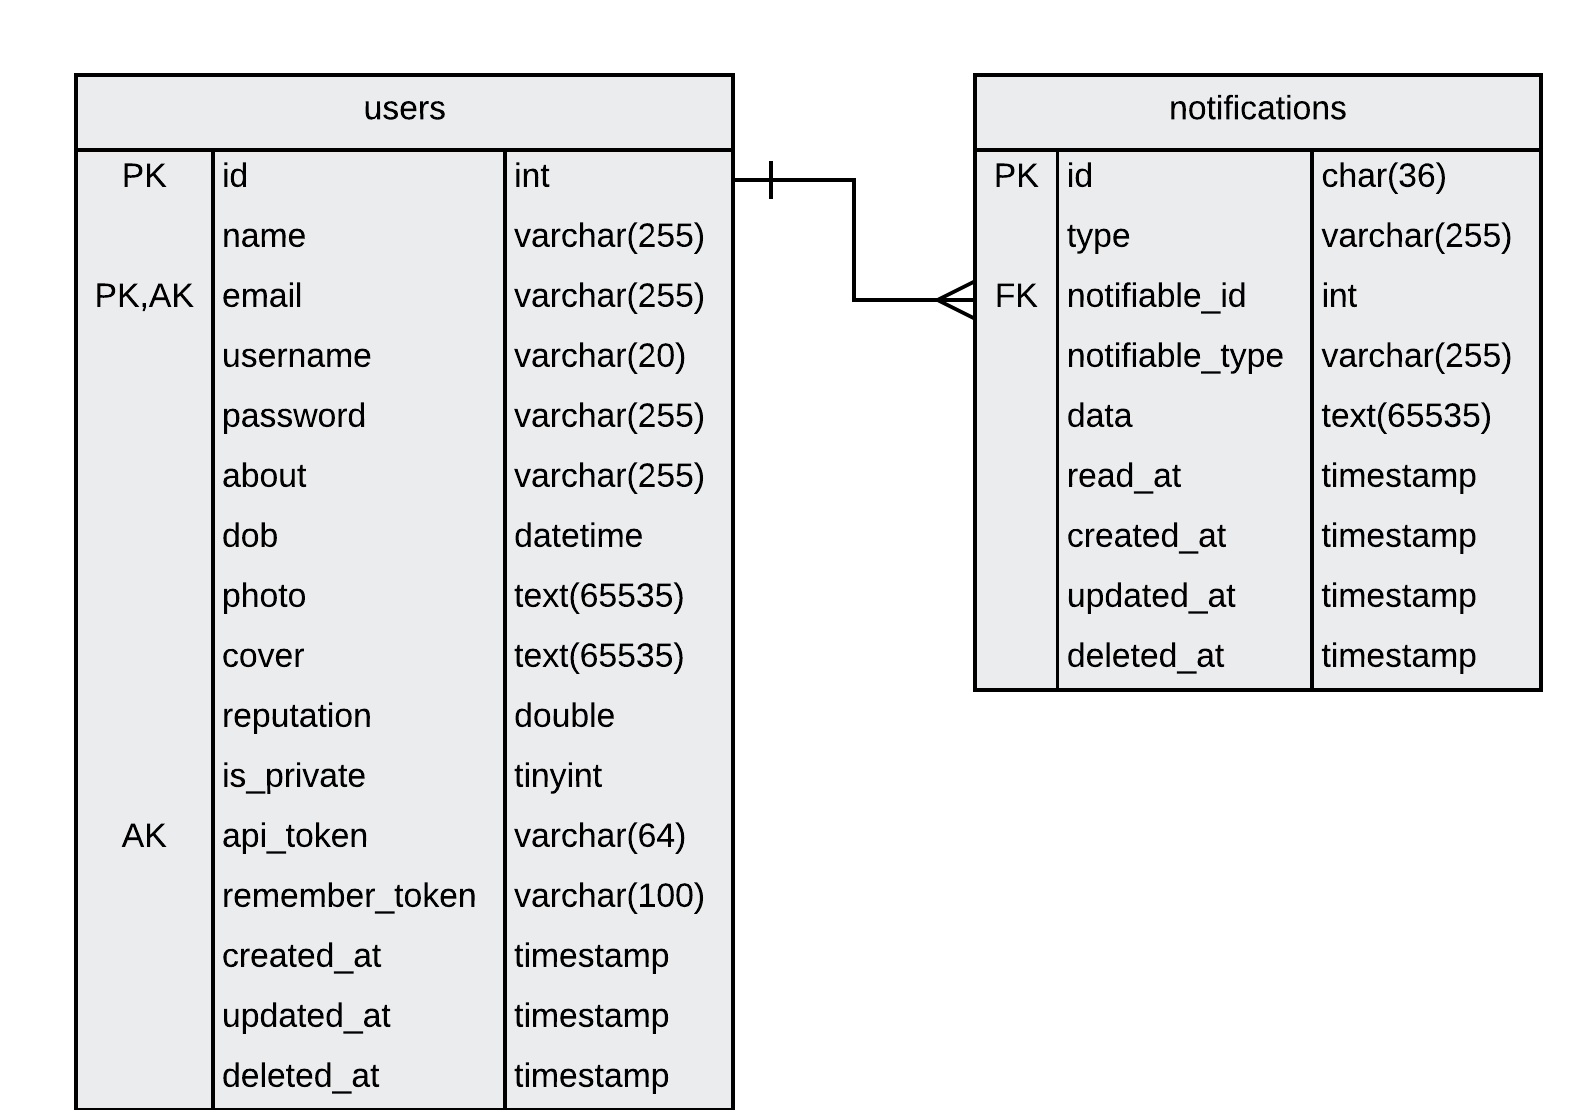
\includegraphics[width=1.0\textwidth]{Images/Design/Database/Notifications}
  \caption{Entity Relationship Diagram - User Notifications} \label{fig:ERD_Notifications}
\end{figure}

\subsubsection{Recommendations}
Recommendations will be used in Fidelis to generate new content for users to explore and interact with. To provide as much variety in recommendations as possible, two recommendation types will be generated (and therefore stored) for users: user and content recommendations. Both tables will need to store the user ID for the user receiving the recommendation, and will also need to store the ID of the recommendation itself (recommended id for users and post id for content). When recommendations are generated, users will not interact with them instantaneously. To monitor recommendation interactions, both tables include a response field which will keep track of a users response to a recommendation (either unread, accepted or rejected). Additionally the content recommendation has a field for tag ID. This ID corresponds to the tag for the post recommendation. Storing this ID provides option for the future use of recommendations. With this field, it will be possible to learn tags users favour and focus on generating recommendations from these. This field could just as easily be used for the opposite reason, and instead aim to generate recommendations outside of the users preferred tags.

\begin{figure}[H]
  \centering
  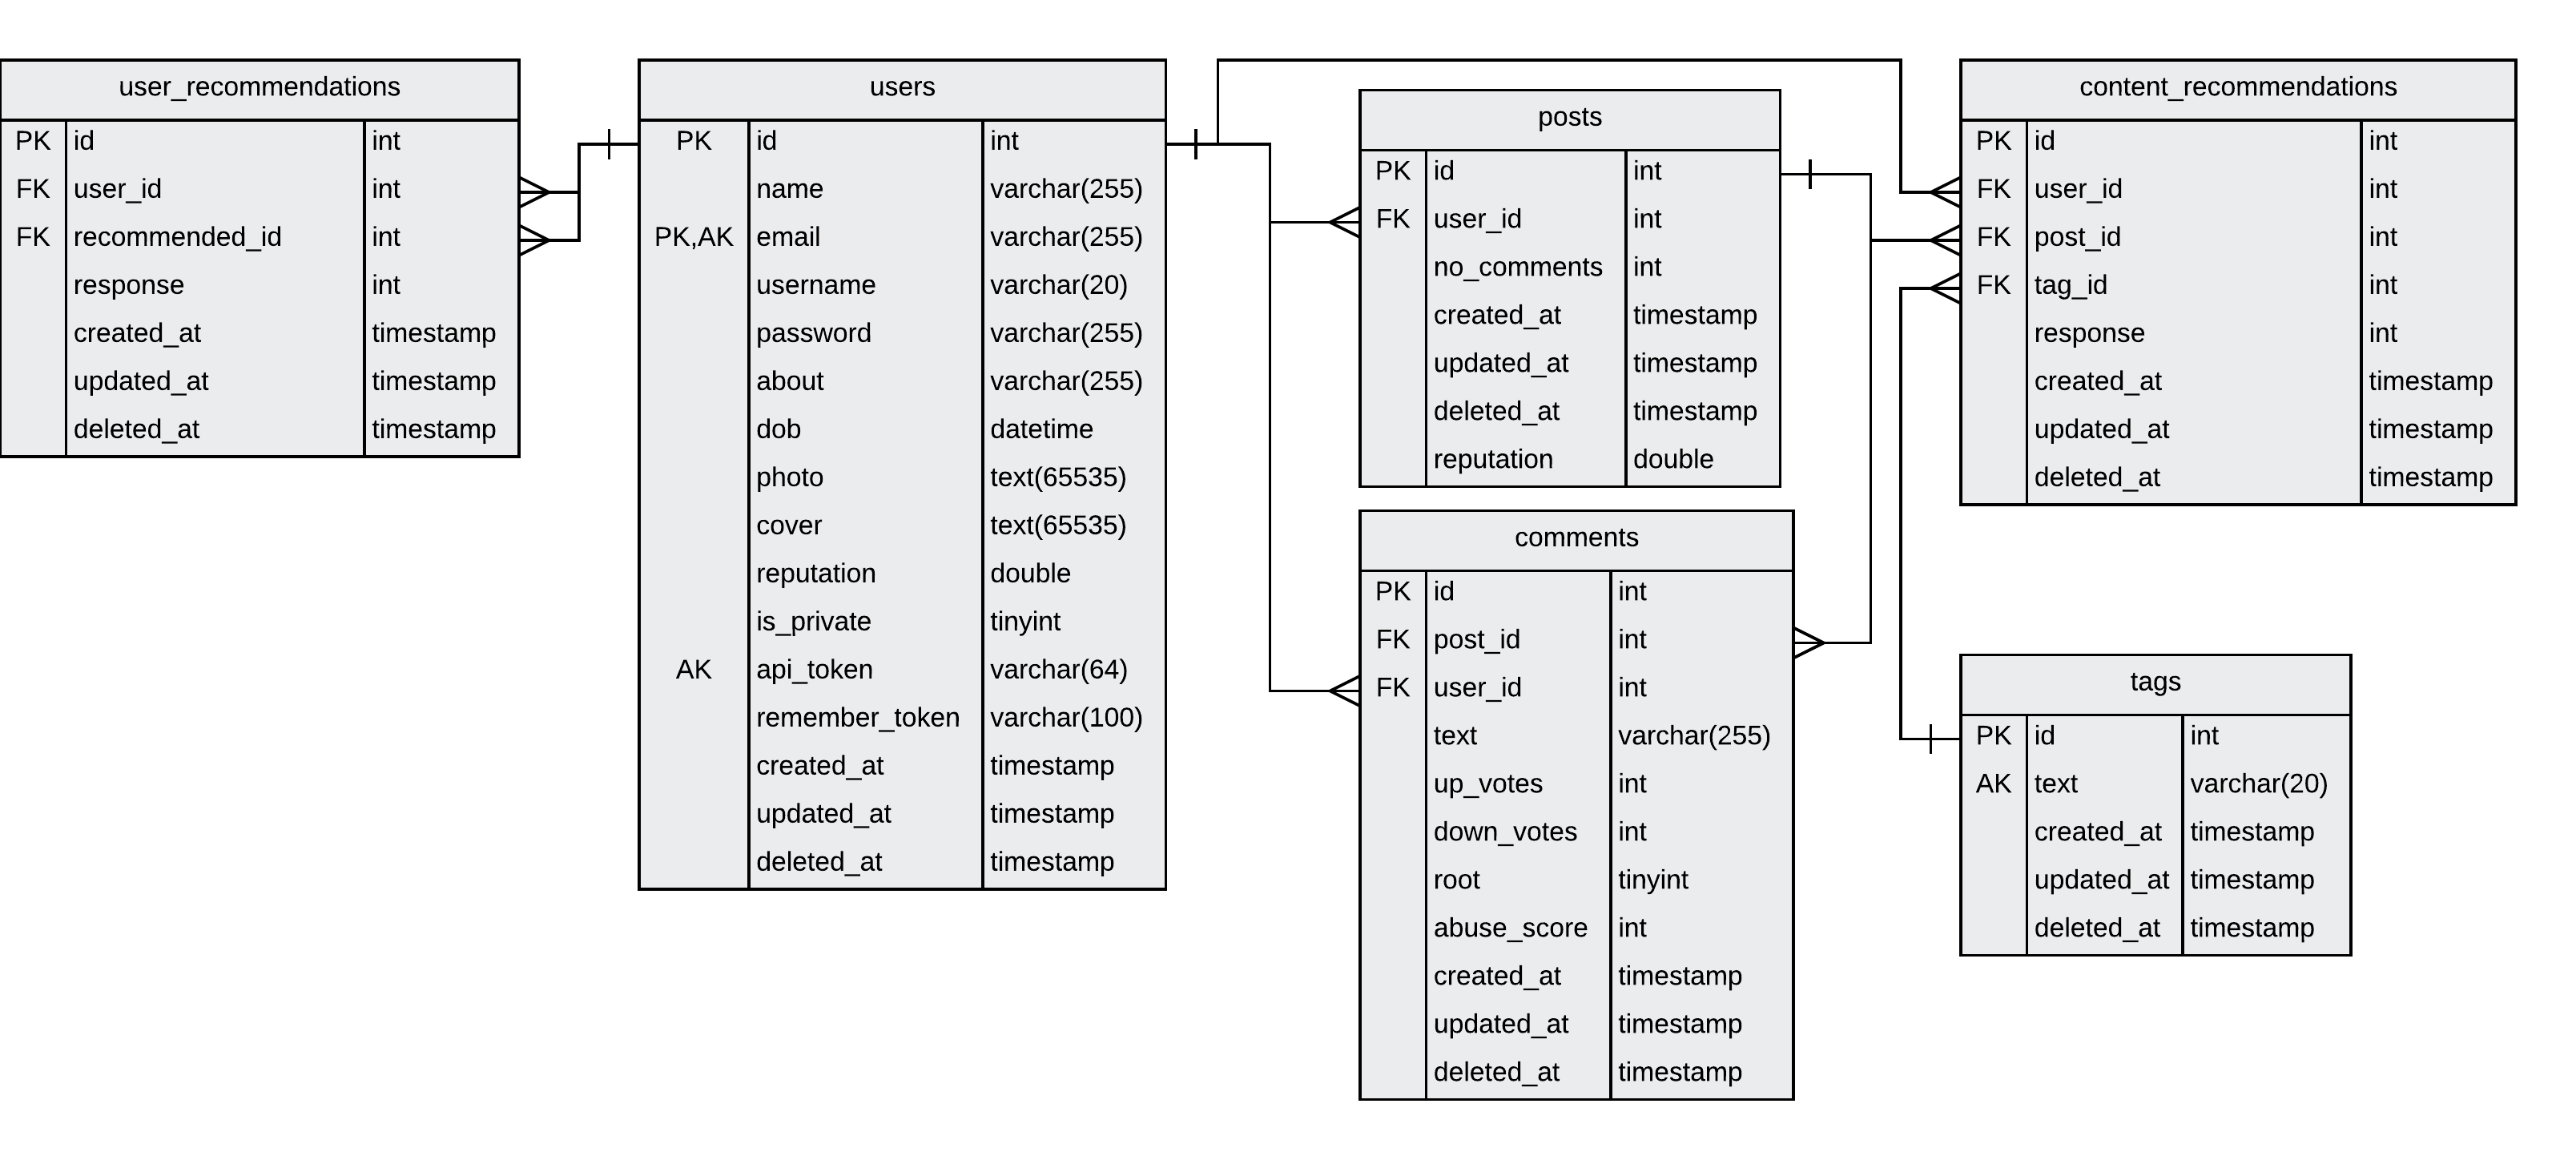
\includegraphics[width=1.0\textwidth]{Images/Design/Database/Recommendations}
  \caption{Entity Relationship Diagram - Personalised Recommendations} \label{fig:ERD_Recommendations}
\end{figure}

\subsubsection{Miscellaneous}
Some tables just store the static data required for the functionality of some pages. These tables are not altered by any of the users. There are two such tables in the database.

\paragraph{Quotes} The quotes table simply stores quotes. Each record is an individual quote and has a text attribute which hold the quote text and a by attribute which hold the authors name.

\paragraph{Wallpapers} The wallpapers table only has one required attribute. The path attribute stores the path to various wallpaper images stored on the server. These can easily be fetched for dynamic background changes on the website.

\begin{figure}[H]
  \centering
  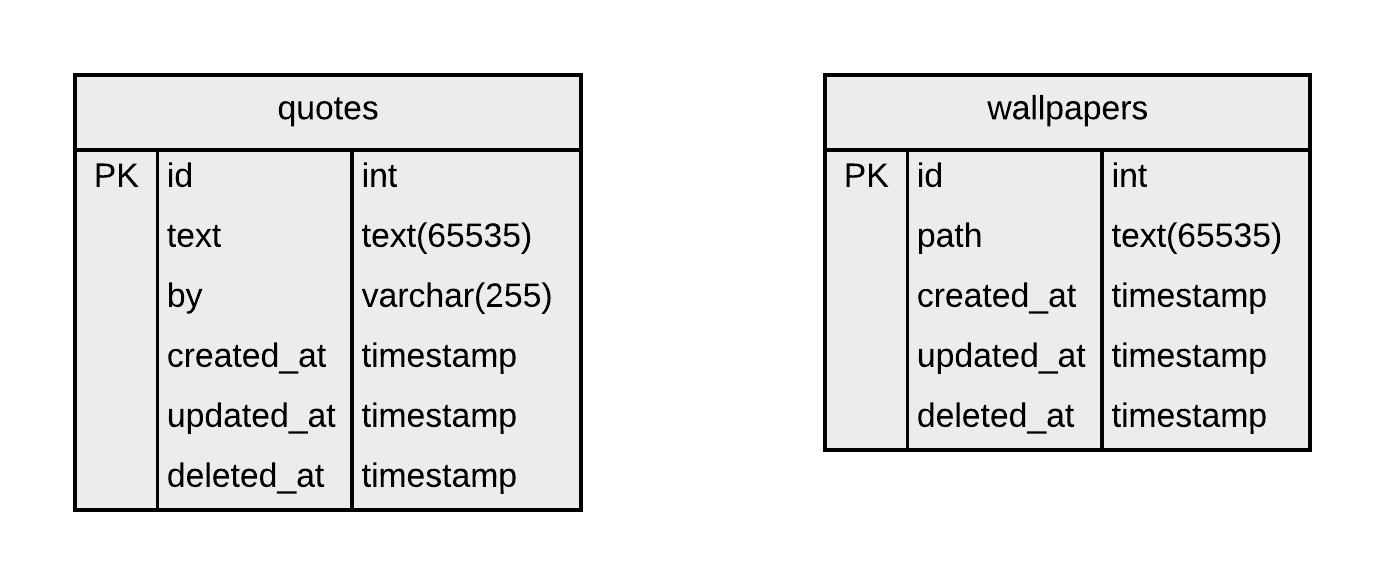
\includegraphics[width=1.0\textwidth]{Images/Design/Database/Miscellaneous}
  \caption{Entity Relationship Diagram - Wallpapers and Quotes} \label{fig:ERD_Miscellaneous}
\end{figure}

\subsection{Normalisation and Redundancy}
\label{SubSection:Database_Normalisation}
``Normalisation is the process of efficiently organising data in a database. There are two goals of the normalisation process: eliminating redundant data and ensuring data dependencies make sense.'' \cite{Databases:NormalisationBasics}. There are various normal forms that a database can be normalised to, starting at first normal form. Each time a database is normalised further it usually results in data being split up into more table and more dependencies being created. The database for the system was normalised to third normal form as this removed all redundant data from the tables whilst providing dependencies that made sense.

\begin{figure}[H]
	\centering
	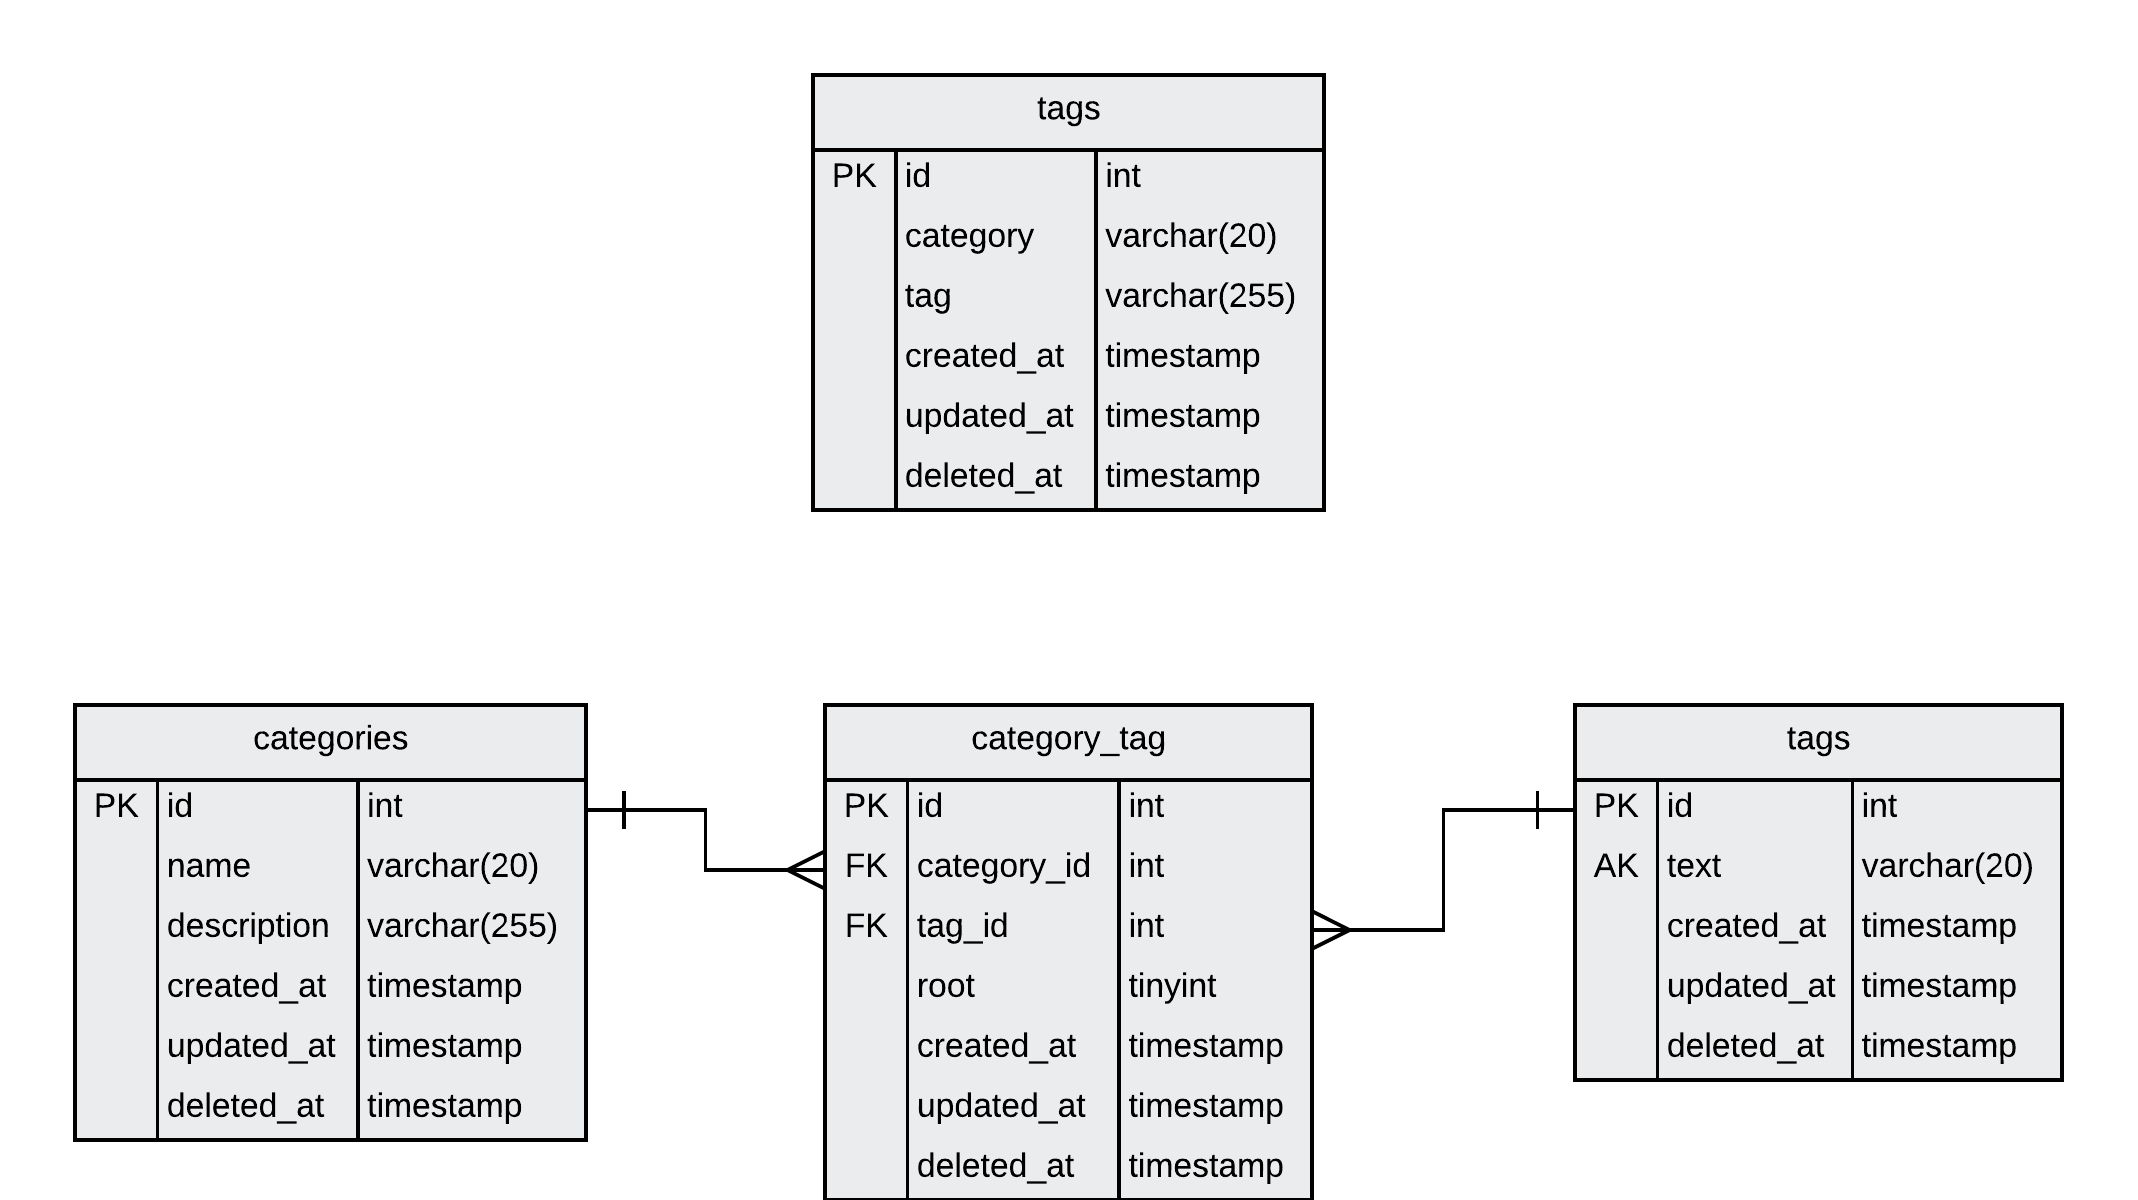
\includegraphics[width=1.0\textwidth]{Images/Design/Database/3NF_Tags}
	\caption{Tags Table - Original vs Third Normal Form} \label{fig:3NF_Tags}
\end{figure}

Third normal form expects that the requirements for all the previous normal forms are met and any columns that are not dependent upon the primary key should be removed \cite{Databases:NormalisationBasics}. Figure \ref{fig:3NF_Tags} shows the original tags table and the same table in third normal form which resulted in three different tables. In this scenario, the category field in the tags table was moved into its own table to reduce redundant information storage and a pivot table was introduced to map tags to categories.

\subsection{Functional Dependencies and Constraints}
\label{SubSection:Database_Constraints}
In a large normalised database with several tables, it is often the case that information in one table relates to information in another table. SQL dependencies are the by-name references, that are used in SQL expressions, that make one entity reliant on another entity \cite{Microsoft:Dependencies}. An entity being referenced by another entity is known as a referenced entity whereas an entity referencing another entity is known as a referencing entity. There are two different types of dependencies that can be introduced into a database.

\begin{itemize}
	\item \textbf{Schema-bound dependency}: A schema-bound dependency is a relationship between two entities that prevents the referenced entity from being dropped or modified as long as the referencing entity exists \cite{Microsoft:Dependencies}.
	\item \textbf{Non-schema-bound dependency}: A non-schema-bound dependency is a relationship between two entities that does not prevent the referenced entity from being dropped or modified \cite{Microsoft:Dependencies}.
\end{itemize}

Dependencies can be defined in an SQL schema when creating tables by using the references keyword which links an attribute in one entity to an attribute in another. This prevents data being inserted into the referencing entity if the exact value for the attribute does not exist in the referenced entity. This feature is known as referential integrity and prevents redundant data building up in the database. Additionally the administrator can specify the effects of a change in the referenced entity.

In the database design, either directly or indirectly, dependencies were used to link all the entities to one another. This can be seen by the links between tables in figure \ref{fig:Database_ERD}. The relationships among these entities vary between a one-to-one relationship and a one-to-many relationship depending on the type of data being stored. For example, a user can have many posts so a one-to-many relationships exists between the users and posts table.